% \documentclass[aspectratio=169, 11pt]{beamer}
\documentclass[aspectratio=169, 11pt, handout]{beamer}

% ── Theme ──
\usetheme{Madrid}
\usecolortheme{default}
\setbeamertemplate{navigation symbols}{}
\setbeamertemplate{footline}{%
  \leavevmode\hbox{%
    \begin{beamercolorbox}[wd=.333333\paperwidth,ht=2.5ex,dp=1ex,center]{author in head/foot}%
      \usebeamerfont{author in head/foot}\insertshortauthor
    \end{beamercolorbox}%
    \begin{beamercolorbox}[wd=.333333\paperwidth,ht=2.5ex,dp=1ex,center]{title in head/foot}%
      \usebeamerfont{title in head/foot}\insertshorttitle
    \end{beamercolorbox}%
    \begin{beamercolorbox}[wd=.333333\paperwidth,ht=2.5ex,dp=1ex,right]{date in head/foot}%
      \usebeamerfont{date in head/foot}\insertframenumber{} / \inserttotalframenumber\hspace*{2ex}
    \end{beamercolorbox}}}

% ── Packages ──
\usepackage{amsmath,amssymb}
\usepackage{booktabs}
\usepackage{xcolor}
\usepackage{colortbl}
\usepackage{graphicx}
\usepackage{tikz}
\usetikzlibrary{arrows.meta, positioning, calc}

% ── Colors ──
\definecolor{sbgreen}{HTML}{00704A}  % course accent
\definecolor{warnred}{HTML}{CC0000}
\definecolor{noteblue}{HTML}{2060A0}

% ── Commands ──
\newcommand{\E}{\mathbb{E}}
\newcommand{\Var}{\mathrm{Var}}
\newcommand{\Cov}{\mathrm{Cov}}
\newcommand{\SE}{\mathrm{SE}}
\newcommand{\Prob}{\mathrm{Pr}}
\newcommand{\indep}{\perp\!\!\!\perp}

\usepackage{soul}
\newcommand{\NUM}[2]{\sethlcolor{yellow}\hl{#1\,\textsuperscript{?}}\marginpar{\tiny #2}}
% Beamer frames are typeset inside boxes, where \marginpar raises "Not in outer par mode"
% and \marginparwidth is 4pt. Same marker; the provenance note goes to the frame footnote.
\renewcommand{\NUM}[2]{\sethlcolor{yellow}\hl{#1\,\textsuperscript{?}}\footnote[frame]{\tiny #2}}
% Compact footnote layout so several provenance notes fit under one frame.
\setbeamertemplate{footnote}{\noindent\raggedright\hspace*{0.6em}\tiny\insertfootnotemark\,\insertfootnotetext\par}

% Version 2 (2026-09-29). Course spine: estimand -> identification -> estimation.
% Changes from slides.tex: m05/CHANGES-v2.md.
\newcommand{\spinestep}[1]{\textcolor{sbgreen}{\textbf{#1}}}

% ── Title ──
\title[Meeting 5]{Meeting 5: What Is the List Worth?}
\subtitle{Applied Causal Inference for Business}
\author{Zhikun Lu}
\date{\today}

\begin{document}

% ====================================================================
\begin{frame}
\titlepage
\end{frame}

% ====================================================================
\begin{frame}{Where Does the Counterfactual Come From?}

\begin{center}
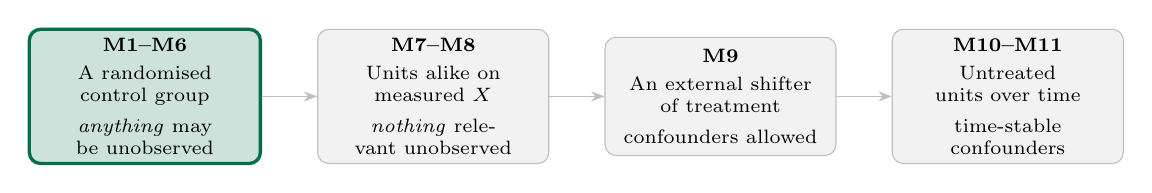
\begin{tikzpicture}[
    node distance=0.45cm and 0.7cm,
    box/.style={draw, rounded corners, minimum width=2.9cm, minimum height=1.5cm,
                font=\scriptsize, align=center, text width=2.7cm},
    active/.style={box, fill=sbgreen!20, draw=sbgreen, very thick},
    inactive/.style={box, fill=gray!10, draw=gray!50}
]
\node[active] (A) {\textbf{M1--M6}\\[2pt] A randomised control group\\[3pt] \emph{anything} may be unobserved};
\node[inactive, right=of A] (B) {\textbf{M7--M8}\\[2pt] Units alike on measured $X$\\[3pt] \emph{nothing} relevant unobserved};
\node[inactive, right=of B] (C) {\textbf{M9}\\[2pt] An external shifter of treatment\\[3pt] confounders allowed};
\node[inactive, right=of C] (D) {\textbf{M10--M11}\\[2pt] Untreated units over time\\[3pt] time-stable confounders};

\draw[-{Stealth}, gray!50] (A) -- (B);
\draw[-{Stealth}, gray!50] (B) -- (C);
\draw[-{Stealth}, gray!50] (C) -- (D);
\end{tikzpicture}
\end{center}

\bigskip

\begin{center}
\small M3 and M4 produced lists. Nobody can observe what a list would have earned for a single customer.\\
The coin, once more, lets us measure it for the whole list --- on rows the list never saw.
\end{center}
\end{frame}

% ====================================================================
\begin{frame}{Today's Plan}

\begin{center}
\small
\begin{tabular}{rp{11.6cm}}
\toprule
\textbf{Minutes} & \\
\midrule
0--15 & \textbf{Reading and critique C3} --- on paper, no devices \\
15--50 & \spinestep{Estimand:} what a frozen list earns. Gain curves, denominators, ranking vs calibration \\
60--110 & The freeze. \spinestep{Identification:} the IPW value identity. \spinestep{Estimation:} row contributions, their SE, \textbf{paired} comparisons; selection vs evaluation; consolidating M1--M5 \\
120--180 & \textbf{Workshop:} contributions, thresholds, selection vs held-out (prediction and hand calculation without AI) \\
\bottomrule
\end{tabular}
\end{center}

\bigskip

\textbf{Case:} Lin's coupon programme, Meeting 5 (Releases 1--4). \quad \textbf{Next meeting:} Exam I (M1--M5). \quad \textbf{Due 72 hours before M7:} project proposal.

\bigskip

\textbf{Reading:} technical notes for Meeting 5.
\end{frame}

% ====================================================================
\begin{frame}{Critique C3: Five Questions, Every Time}

Read the one-page case silently. Notes on your own, then pairs, then the room.

\bigskip

\begin{enumerate}
    \item What is the claim?
    \item What causal question does the decision need?
    \item Who is the comparison group?
    \item What else could produce this pattern? Give the mechanism and the \textbf{direction} of the bias.
    \item What would you do to find out?
\end{enumerate}

\bigskip

\small C3's flaw is a Meeting 4 idea. Ask of any number: was it computed on the data that chose it? Hand in your notes at minute 15.
\end{frame}

% ====================================================================
\section{The Estimand: What a Frozen List Earns}
% ====================================================================

% [RELEASE R1 — the three candidate lists; evaluation-fold outcomes stay locked]
% [RELEASE R1 — the three candidate lists; evaluation-fold outcomes stay locked]
\begin{frame}[shrink=5]{Three Lists, One Launch}

The 5{,}000 Q3 coupons (M3) go out next month. The chain has licensed an \textbf{automated campaign engine}: it builds lists from the Q2 export and would send them itself. Three lists are on Lin's desk, each built on the training folds:

\begin{center}
\begin{tabular}{lp{7.6cm}}
\toprule
\textbf{List} & \textbf{How it was built} \\
\midrule
Segment rule & All lapsed members (M1). No model. \\
T-learner & Top 5{,}000 by $\widehat\tau(x)$ from boosted arm models (M3) --- the engine \\
Causal forest & Top 5{,}000 by the forest's $\widehat\tau(x)$ (M4) --- the engine \\
\bottomrule
\end{tabular}
\end{center}

The engine also offers to choose its own cut-off.

\bigskip

\textbf{The CFO asks one question:} \emph{what will each list earn, compared with sending nothing?} And sets one rule: \textbf{nothing the engine proposes goes live until it is frozen and valued on a fold of the Q2 test it has never seen}.

\medskip

\small An automated system that decides who gets what is still a policy. It is evaluated like any other.
\end{frame}

% ====================================================================
\begin{frame}{The Number That Decides It}

A list is a policy $\pi(x) \in \{0, 1\}$. From M3, a coupon to member $x$ earns $\text{net}(x) = 30\,\tau(x) - 10\,\mu_1(x)$. The list's \textbf{gain} over sending nothing, per member of the base:

\begin{alertblock}{Policy gain}
\[
G(\pi) \;=\; \E\bigl[\pi(X)\,\text{net}(X)\bigr]
\]
\end{alertblock}

\pause

Two lists we can price by hand, on the M1 base of 10{,}000:

\begin{center}
\small
\begin{tabular}{lrr}
\toprule
\textbf{List} & \textbf{Gain per member} & \textbf{Total} \\
\midrule
Coupon nobody & 0 & 0 \\
Coupon everyone & $\tfrac12(-6.50) + \tfrac12(3.00) = -$\textyen 1.75 & $-$\textyen 17{,}500 \\
Segment rule (lapsed) & $\tfrac12(3.00) = +$\textyen 1.50 & $+$\textyen 15{,}000 \\
\bottomrule
\end{tabular}
\end{center}

\medskip

Every estimate today is a policy gain. The only question is whether a model's list \textbf{beats \textyen 1.50} --- the list that needed no model.
\end{frame}

% ====================================================================
\begin{frame}{Three Steps for a Policy}

\begin{center}
\small
\begin{tabular}{p{2.8cm}p{9.8cm}}
\toprule
\spinestep{Estimand} & $G(\pi) = \E[\pi(X)\,\text{net}(X)]$ for a \textbf{frozen} list $\pi$: what it earns per member of the base, against sending nothing. A property of the list, not of any model inside it. \\[0.5em]
\spinestep{Identification} & A fold of the Q2 test with its coin intact. Because $e = 0.5$ is \emph{known}, weighting the rows where the coin agreed with the list reconstructs $G(\pi)$ exactly (the IPW identity, section 3). \\[0.5em]
\spinestep{Estimation} & The average of row contributions; its SE from the same rows; for two lists, \textbf{paired} differences on the same rows. \\
\bottomrule
\end{tabular}
\end{center}

\bigskip

Two things break the chain: a list that is \emph{not} frozen (it can be tuned to the fold's noise), and a fold whose coin has been disturbed.
\end{frame}

% ====================================================================
\section{Estimation: Gain Curves}
% ====================================================================

\begin{frame}{The Targeting Depth Curve}

Rank all members by $\widehat\tau(x_i)$, descending. As the list grows, the ATT of the treated falls --- and so does the money:

\bigskip

\begin{center}
\small
\begin{tabular}{lcccr}
\toprule
\textbf{Depth} $k$ & \textbf{Who is on the list} & $\tau_{S_k}$ & \textbf{Interpretation} & \textbf{Net (\textyen)} \\
\midrule
1{,}000 & 1{,}000 lapsed & 0.20 & Highest-effect only & $+$3{,}000 \\
5{,}000 & All lapsed & 0.20 & All high-effect members & $+$15{,}000 \\
7{,}500 & Lapsed $+$ 2{,}500 active & 0.15 & Diluted by active & $-$1{,}250 \\
10{,}000 & Everyone & 0.125 & $=$ ATE & $-$17{,}500 \\
\bottomrule
\end{tabular}
\end{center}

\bigskip

The lift at depth 7{,}500 is still $0.15$; the list already loses money. \textbf{A lift curve is not a profit curve.}

\medskip

If the ranking is corrupted (noisy, biased), we treat the wrong people and $\tau_{S_k}$ is lower at every depth.
\end{frame}

% [CARRIED VERBATIM from old-decks/lecture04.tex:110]
\begin{frame}{Ranking Quality Is What Matters}
 
Sometimes, the business value of CATE estimation depends on how well $\hat{\tau}(x)$ \emph{ranks} customers, not on the accuracy of individual point estimates.
 
\bigskip
 
A model with correct rankings but wrong magnitudes produces a better targeting rule than a model with accurate magnitudes but poor rankings.
 
\bigskip
 
$\Rightarrow$ We need an \textbf{evaluation framework} for CATE rankings.
 
\end{frame}

% [CARRIED VERBATIM from old-decks/lecture04.tex:147]
\begin{frame}{The Evaluation Problem}
 
\textbf{Standard ML:} Compare predictions to observed labels.
\begin{itemize}
    \item Accuracy, AUC, RMSE, \ldots
    \item Ground truth exists for every observation
\end{itemize}
 
\bigskip
 
\textbf{Causal ML:} The \emph{label} $\tau_i = Y_i(1) - Y_i(0)$ is \textbf{never observed}.
 
\begin{itemize}
    \item We see $Y_i(1)$ or $Y_i(0)$, never both $\Longrightarrow$ ground truth $\tau_i$ never known
    \item Cannot compute $\frac{1}{n}\sum_i (\hat{\tau}(x_i) - \tau_i)^2$
\end{itemize}
 
\bigskip
 
\begin{alertblock}{Key Insight}
Evaluate the \textbf{quality of the targeting decisions}, not the accuracy of point estimates. Use \textbf{group-level} experimental comparisons.
\end{alertblock}
\end{frame}

% [CARRIED VERBATIM from old-decks/lecture04.tex:172]
\begin{frame}{The Thought Experiment}
 
Suppose a model ranks customers by $\hat{\tau}(x_i)$ from highest to lowest.
 
\bigskip
 
\textbf{Question:} If we send coupons to the top $k\%$ of customers, what is the treatment effect in that group?
 
\bigskip
 
\textbf{A good model should:}
\begin{itemize}
    \item Put high-CATE customers at the top $\Rightarrow$ large effect in top group
    \item Put low/negative-CATE customers at the bottom $\Rightarrow$ small or negative effect
\end{itemize}
 
\bigskip
 
\textbf{A random ranking:} the effect in the top $k\%$ equals the ATE regardless of $k$. This gives us a \textbf{baseline}.
\end{frame}

% ====================================================================
% [REPLACES the schematic gain curve: common endpoint, exact example]
\begin{frame}{The Gain Curve}

Four equal groups with true effects $0.20, 0.10, 0.00, -0.10$ (ATE $= 0.05$). Target a fraction $q$; plot incremental purchases \textbf{per member of the base}, $G(q) = q \times$ (lift among the targeted).

\begin{columns}[T]
\begin{column}{0.46\textwidth}
\footnotesize
\begin{tabular}{lrrrr}
\toprule
$q$ & .25 & .50 & .75 & 1 \\
\midrule
Best ranking & .050 & .075 & .075 & .050 \\
Random & .0125 & .025 & .0375 & .050 \\
Worst ranking & $-.025$ & $-.025$ & 0 & .050 \\
\bottomrule
\end{tabular}
\end{column}
\begin{column}{0.52\textwidth}
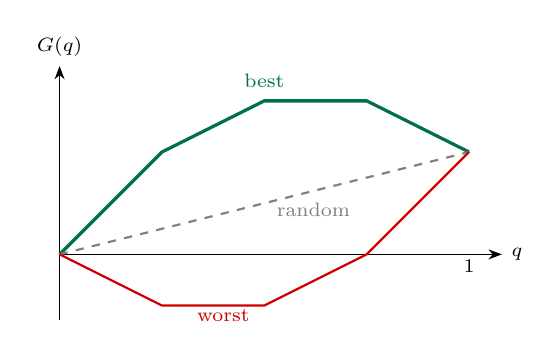
\begin{tikzpicture}[x=5.2cm, y=26cm]
\draw[-{Stealth}] (0,0) -- (1.08,0) node[right, font=\scriptsize] {$q$};
\draw[-{Stealth}] (0,-0.032) -- (0,0.092) node[above, font=\scriptsize] {$G(q)$};
\draw[sbgreen, very thick] (0,0) -- (0.25,0.05) -- (0.5,0.075) -- (0.75,0.075) -- (1,0.05);
\draw[gray, dashed, thick] (0,0) -- (1,0.05);
\draw[warnred, thick] (0,0) -- (0.25,-0.025) -- (0.5,-0.025) -- (0.75,0) -- (1,0.05);
\node[font=\scriptsize, sbgreen] at (0.5,0.085) {best};
\node[font=\scriptsize, gray] at (0.62,0.022) {random};
\node[font=\scriptsize, warnred] at (0.4,-0.03) {worst};
\node[font=\scriptsize] at (1,-0.006) {1};
\end{tikzpicture}
\end{column}
\end{columns}

\bigskip

\textbf{Every ranking ends at the same point}: at $q = 1$ everyone is treated and the gain is the ATE. A good ranking rises steeply, then \emph{falls} once it reaches the groups the coupon does not help. The curve measures \emph{purchases}, not money: the redemption cost is not on it.
\end{frame}

% ====================================================================
% [RELEASE R2 — the top-20% group on the evaluation fold; worksheet before the reveal]
\begin{frame}{Denominators}

Within the top $\phi$, arms are \emph{random}, not equal. The top 20\% of an evaluation fold of 5{,}000:

\begin{center}
\small
\begin{tabular}{lrrr}
\toprule
& \textbf{Members} & \textbf{Bought} & \textbf{Rate} \\
\midrule
Coupon arm & 540 & 216 & 0.40 \\
Control arm & 460 & 138 & 0.30 \\
\bottomrule
\end{tabular}
\end{center}

\pause

\begin{center}
\small
\begin{tabular}{lr}
\toprule
Count difference: $216 - 138$ & \textcolor{warnred}{78} \\
Rate difference $\times$ members: $(0.40 - 0.30) \times 1{,}000$ & \textcolor{sbgreen}{100} \\
\bottomrule
\end{tabular}
\end{center}

\smallskip

The count difference answers no question. Compute each arm's \textbf{rate}, then scale.
\vspace{-0.5em}
\[
78 = 540(0.40) - 460(0.30) = \underbrace{50}_{\text{half the group couponed}} + \underbrace{28}_{\text{arm sizes differ}}
\]
\vspace{-1.2em}

\pause

\small Three denominators: lift per member \emph{targeted} ($0.10$); per member of the \emph{base}, $Q(0.2) = 0.02$; profit per \emph{coupon}. Use the one the decision uses.
\end{frame}

% [CARRIED VERBATIM from old-decks/lecture04.tex:248]
\begin{frame}{AUUC: Area Under the Uplift Curve}
 
\begin{block}{AUUC}
\[
\text{AUUC} = \int_0^1 \bigl[Q(\phi) - \phi \cdot \text{ATE}\bigr] \, d\phi
\]
\end{block}
 
\bigskip
 
\begin{itemize}
    \item AUUC $> 0$: model is better than random targeting
    \item AUUC $= 0$: model is no better than random
    \item AUUC $< 0$: model is worse than random (inverted ranking)
\end{itemize}
 
\bigskip
 
\textbf{Analogy:} AUUC is to CATE evaluation what AUC-ROC is to classification.

\medskip
\small By hand, on the four groups: the best ranking's gain above random is $0, .0375, .05, .0375, 0$ at $q = 0, .25, \ldots, 1$; the trapezoids give an area of $\mathbf{0.03125}$. A ranking summary --- not campaign profit.
\end{frame}

% [CARRIED VERBATIM from old-decks/lecture04.tex:270]
\begin{frame}[shrink=6]{Comparing Models with Qini Curves}
 
\begin{center}
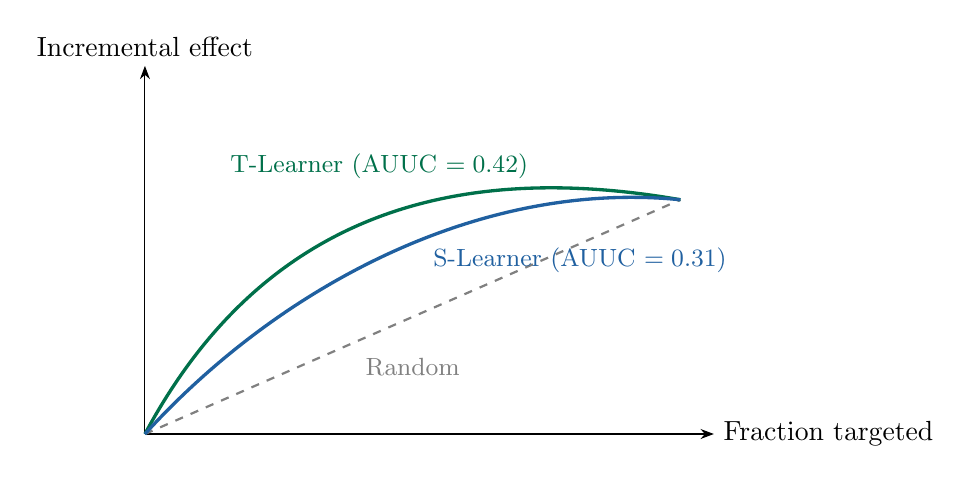
\begin{tikzpicture}[scale=0.85]
% Axes
\draw[-{Stealth}] (0,0) -- (8.5,0) node[right] {Fraction targeted};
\draw[-{Stealth}] (0,0) -- (0,5.5) node[above] {Incremental effect};
 
% Random baseline
\draw[gray, dashed, thick] (0,0) -- (8,3.5);
 
% T-Learner
\draw[sbgreen, very thick] (0,0) .. controls (1.5,2.8) and (4,4.2) .. (8,3.5);
\node[sbgreen, font=\small] at (3.5, 4.0) {T-Learner (AUUC $= 0.42$)};
 
% S-Learner
\draw[noteblue, very thick] (0,0) .. controls (2,2.2) and (5,3.8) .. (8,3.5);
\node[noteblue, font=\small] at (6.5, 2.6) {S-Learner (AUUC $= 0.31$)};
 
\node[gray, font=\small] at (4,1.0) {Random};
\end{tikzpicture}
\end{center}
 
\bigskip
 
Higher Qini curve $=$ better prioritization of high-CATE customers.
 
\bigskip
 
\textbf{Is the difference meaningful or noise?} Both curves use the \emph{same} evaluation members, so the comparison must be \textbf{paired} (section 3).
\end{frame}

% [CARRIED VERBATIM from old-decks/lecture04.tex:354]
\begin{frame}{Calibration: Rankings Are Not Enough}
 
AUUC and RATE evaluate \textbf{ranking quality}. They say \textbf{nothing about magnitudes}.
 
\bigskip
 
A model predicting $\hat{\tau}(x) \in \{10, 20\}$ when true effects are $\tau(x) \in \{1, 2\}$ would rank perfectly but overstate effects by 10$\times$.
 
\bigskip
 
\textbf{Why this matters:} a marketing team projecting campaign ROI needs correct magnitudes, not just correct rankings.
\end{frame}

% [CARRIED VERBATIM from old-decks/lecture04.tex:368]
\begin{frame}{The CATE Reliability Diagram}
 
\textbf{Procedure:}
\begin{enumerate}
    \item Bin customers by predicted CATE ($K$ groups by quantile)
    \item Within each bin, estimate actual ATE: $\hat{\tau}_k = \bar{Y}_{1,k} - \bar{Y}_{0,k}$
    \item Plot mean predicted CATE vs.\ estimated actual ATE
\end{enumerate}
 
\bigskip
 
\begin{center}
\begin{tabular}{lcc}
\toprule
\textbf{Bin} & \textbf{Mean predicted} $\hat{\tau}$ & \textbf{Estimated actual} $\hat{\tau}_k$ \\
\midrule
Bottom 20\% & $-2.1\%$ & $-0.5\% \pm 1.8\%$ \\
40--60\% & $+8.2\%$ & $+7.5\% \pm 1.7\%$ \\
Top 20\% & $+25.3\%$ & $+16.8\% \pm 2.4\%$ \\
\bottomrule
\end{tabular}
\end{center}
 
\bigskip
 
Rankings are good (actual effects increase monotonically), but the top bin is substantially overestimated. \textbf{Fix:} isotonic regression recalibrates while preserving rankings.
\end{frame}

% ====================================================================
% [RELEASE R3 — the freeze: predictions file and code snapshot collected]
\begin{frame}{Freeze, Then Evaluate}

From the CFO's rules for the evaluation fold --- the rules every list from the engine must pass:

\bigskip

\begin{center}
\small
\begin{tabular}{p{6.4cm}p{6.6cm}}
\toprule
\textbf{The case says} & \textbf{Which buys} \\
\midrule
``The evaluation fold was drawn at random from the Q2 export before any model was fitted.'' & The fold is a random sample of the base: its value speaks for the base. \\[0.4em]
``Its 50/50 coupon draw is intact.'' & $e = 0.5$ is \emph{known}: the IPW identity is exact, not modelled. \\[0.4em]
``Its outcomes are released only after each list is frozen: a file of $\pi(x_i)$ for every fold member and a timestamped code snapshot.'' & The list cannot have been tuned to the fold's noise. \\
\bottomrule
\end{tabular}
\end{center}

\bigskip
\pause

The third sentence is M4's honesty rule, applied to a \emph{policy} instead of a partition. A list adjusted after one look at the fold is not being evaluated; it is being fitted.
\end{frame}

% ====================================================================
\section{Identification and Estimation: What a Policy Is Worth}
% ====================================================================

\begin{frame}{Policy Value: The IPW Identity}

A member's profit under decision $d$: $r(d) = (30 - 10d)\,Y(d)$ --- \textyen 30 per purchase, less the coupon if one was sent.

\begin{block}{The identity (known $e = 0.5$)}
\vspace{-0.5em}
\[
V(\pi) \equiv \E\bigl[r(\pi(X))\bigr] \;=\; \E\!\left[\frac{\mathbf{1}\{D = \pi(X)\}}{0.5}\; r(D)\right]
\]
\end{block}

\pause

\textbf{Why.} By consistency, the observed $r(D)$ equals $r(\pi(X))$ on the rows where the coin agreed with the list. Given $X$ the coin agrees with probability $0.5$, independently of the potential outcomes; dividing by $0.5$ puts those rows back at full weight.

\pause
\medskip

\textbf{The gain} over sending nothing, as one row contribution:
\[
g_i \;=\; \pi(X_i)\left\{\frac{D_i\, 20\,Y_i}{0.5} - \frac{(1 - D_i)\, 30\,Y_i}{0.5}\right\},
\qquad
\widehat G(\pi) = \frac{1}{n}\sum_i g_i .
\]

\small Only listed members contribute. A coupon-arm buyer adds $40$; a control-arm buyer subtracts $60$. With a different coin, use the design's $e$: at $e = 0.25$ the same buyers contribute $+80$ and $-40$.
\end{frame}

% ====================================================================
% [Worksheet: pairs compute both policies' gains from the cell counts before the next frame]
\begin{frame}{Row Contributions}

A small evaluation fold of 80 members, 50/50 within each segment:

\begin{center}
\small
\begin{tabular}{llrrr}
\toprule
\textbf{Segment} & \textbf{Arm} & \textbf{Members} & \textbf{Bought} & \textbf{$g_i$ per buyer (if listed)} \\
\midrule
Lapsed & coupon & 20 & 6 & $+40$ \\
Lapsed & control & 20 & 2 & $-60$ \\
Active & coupon & 20 & 16 & $+40$ \\
Active & control & 20 & 15 & $-60$ \\
\bottomrule
\end{tabular}
\end{center}

\smallskip
\small Non-buyers contribute 0. Members off the list contribute 0.

\bigskip
\normalsize

\textbf{In pairs:} $\widehat G$ for (a) the segment rule, (b) coupon everyone, (c) coupon the active only. Which is closest to the hand values of the previous section?
\end{frame}

% ====================================================================
\begin{frame}{The Contributions, Added Up}

\begin{center}
\small
\begin{tabular}{lrrr}
\toprule
\textbf{List} & \textbf{Lapsed rows} & \textbf{Active rows} & $\widehat G$ \textbf{per member} \\
\midrule
Segment rule & $6(40) - 2(60) = 120$ & 0 & $120/80 = \textcolor{sbgreen}{1.50}$ \\
Coupon everyone & 120 & $16(40) - 15(60) = -260$ & $-140/80 = \textcolor{warnred}{-1.75}$ \\
Active only & 0 & $-260$ & $-260/80 = \textcolor{warnred}{-3.25}$ \\
\bottomrule
\end{tabular}
\end{center}

\smallskip
\small The fold's rates are exactly the M1 segment rates, so the estimates equal the hand values.

\pause
\medskip
\normalsize

\textbf{How precise?} The segment rule's 80 contributions are six $40$s, two $-60$s and 72 zeros:
\[
\text{sd}(g_i) = 14.5, \qquad \widehat\SE\bigl(\widehat G\bigr) = 14.5/\sqrt{80} = 1.62 .
\]

The estimate is $1.50 \pm 3.2$. Each row carries a large $\pm$ because the coin put it on only one side. At the evaluation fold's real size this shrinks with $\sqrt n$ --- but it never vanishes, and two lists that differ by less than a couple of SEs have not been told apart.
\end{frame}

% ====================================================================
\begin{frame}{Comparing Two Lists: Pair the Rows}

Two frozen lists valued on the \textbf{same} evaluation members. Their estimates share rows, so they are correlated --- usually strongly, when the lists overlap.

\bigskip

\begin{block}{Paired difference}
\[
\widehat\Delta_{A-B} = \frac{1}{n}\sum_i \bigl(g_{A,i} - g_{B,i}\bigr), \qquad
\widehat\SE\bigl(\widehat\Delta\bigr) = \frac{\text{sd}(g_{A,i} - g_{B,i})}{\sqrt n}
\]
\end{block}

\bigskip

\textbf{By hand.} Four evaluation units with paired differences $(0.02,\, 0.00,\, 0.01,\, -0.01)$:
\[
\bar d = 0.005, \qquad \text{sd} = \sqrt{0.0005/3} = 0.0129, \qquad \widehat\SE = 0.0129/2 = 0.0065 .
\]
The interval $0.005 \pm 0.013$ crosses zero. (Four rows show the arithmetic; they are far too few to act on.)

\bigskip

\textbf{Do not} combine the two lists' separate SEs as if they were independent: rows the lists share contribute the same noise to both, and it cancels in the difference.
\end{frame}

% [CARRIED VERBATIM from old-decks/lecture04.tex:417]
\begin{frame}{AUUC vs.\ Policy Value}
 
\textbf{AUUC} asks: does this model \emph{rank} well?
 
\bigskip
 
\textbf{Policy value} asks: what happens if we actually \emph{deploy} this model?
 
\bigskip
 
These can diverge. A model with high AUUC but poor calibration might recommend treating a group whose true effects do not justify the cost.
 
\bigskip
 
\textbf{Evaluate both} for a complete picture.
\end{frame}

% [CARRIED VERBATIM from old-decks/lecture04.tex:460]
\begin{frame}{Honest Evaluation: The Problem}
 
\begin{alertblock}{Critical Point}
If the same data is used to (1) train the model and (2) evaluate it, the Qini curve is \textbf{optimistically biased}.
\end{alertblock}
 
\bigskip
 
The model overfits to noise in the training data, and the evaluation rewards that overfitting.
 
\bigskip
 
This is exactly analogous to reporting training-set AUC in classification.
\end{frame}

% ====================================================================
\begin{frame}{Evaluation Data Roles}

Three row sets, three jobs --- M3's fit/choose/assess, now with a policy in the middle:

\begin{center}
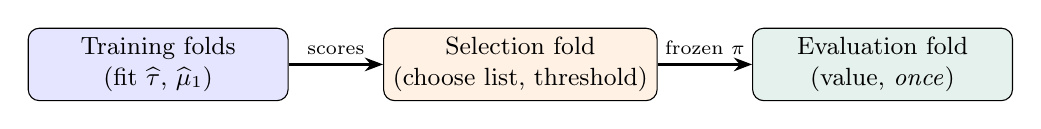
\begin{tikzpicture}[
    box/.style={draw, rounded corners, minimum width=3.3cm, minimum height=0.9cm, font=\small, align=center}
]
\node[box, fill=blue!10] (train) at (0,0) {Training folds\\(fit $\widehat\tau$, $\widehat\mu_1$)};
\node[box, fill=orange!10] (sel) at (4.6,0) {Selection fold\\(choose list, threshold)};
\node[box, fill=sbgreen!10] (eval) at (9.2,0) {Evaluation fold\\(value, \emph{once})};
\draw[-{Stealth}, thick] (train) -- (sel) node[midway, above, font=\scriptsize] {scores};
\draw[-{Stealth}, thick] (sel) -- (eval) node[midway, above, font=\scriptsize] {frozen $\pi$};
\end{tikzpicture}
\end{center}

\bigskip
\pause

\begin{itemize}
    \item The \textbf{selection} fold is where you compare candidates and pick a cut-off. Whatever wins there was chosen \emph{partly on that fold's noise} --- M4's winner's curse, for policies.
    \item The \textbf{evaluation} fold prices the frozen winner. Touch it once; a second look makes it a selection fold.
    \item The engine gets no exception: its cut-off, tuned on the selection fold, is frozen like everything else before the evaluation fold opens.
\end{itemize}
\end{frame}

% ====================================================================
% [RELEASE R4 — the evaluation fold is unlocked]
\begin{frame}{Lin's Table}

Gain per member of the base, \textyen. The simulation's truth is revealed in the workshop.
\vspace{-0.3em}
\begin{center}
\small
\begin{tabular}{lrr}
\toprule
\textbf{List} & \textbf{Selection fold} & \textbf{Evaluation fold (SE)} \\
\midrule
Segment rule (lapsed) & \NUM{1.46}{sim v2: selection-fold gain, lapsed rule} & \NUM{1.53 (0.21)}{sim v2: evaluation gain (SE), lapsed rule} \\
T-learner, top 5{,}000 & \NUM{1.88}{sim v2: selection-fold gain, T-learner list} & \NUM{1.61 (0.22)}{sim v2: evaluation gain, T-learner} \\
Forest, top 5{,}000 & \NUM{2.07}{sim v2: selection-fold gain, forest list} & \NUM{1.79 (0.21)}{sim v2: evaluation gain, forest} \\
Forest, cut-off tuned on selection fold & \textbf{\NUM{2.31}{sim v2: selection-fold gain, forest with tuned cut-off}} & \NUM{1.82 (0.23)}{sim v2: evaluation gain, tuned forest} \\
\bottomrule
\end{tabular}
\end{center}

\pause
\vspace{-0.4em}
\small The more a list was tuned on the selection fold, the more it fell on the evaluation fold. Is the forest's $0.26$ edge over the segment rule real? Only the \textbf{paired} SE of the difference can say: \NUM{?}{sim v2: paired SE of forest-list minus segment-rule gain on the evaluation fold}.
\vspace{0.6em}
\end{frame}

% [CARRIED VERBATIM from old-decks/lecture04.tex:503]
\begin{frame}{The Full Pipeline}
 
\begin{center}
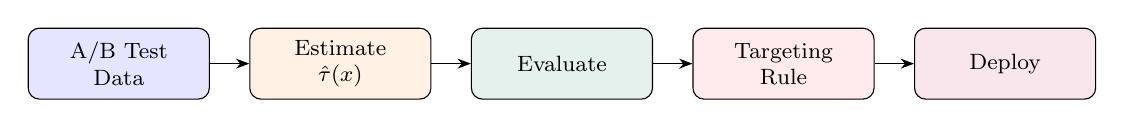
\begin{tikzpicture}[
    node distance=0.6cm and 0.5cm,
    box/.style={draw, rounded corners, minimum width=2.3cm, minimum height=0.9cm, font=\footnotesize, align=center},
]
\node[box, fill=blue!10] (data) {A/B Test\\Data};
\node[box, fill=orange!10, right=of data] (est) {Estimate\\$\hat{\tau}(x)$};
\node[box, fill=sbgreen!10, right=of est] (eval) {Evaluate};
\node[box, fill=red!8, right=of eval] (target) {Targeting\\Rule};
\node[box, fill=purple!10, right=of target] (deploy) {Deploy};
 
\draw[-{Stealth}] (data) -- (est);
\draw[-{Stealth}] (est) -- (eval);
\draw[-{Stealth}] (eval) -- (target);
\draw[-{Stealth}] (target) -- (deploy);
\end{tikzpicture}
\end{center}
 
\bigskip
 
\textbf{Estimate:} S-Learner, T-Learner, causal forest, \ldots
 
\textbf{Evaluate:} Ranking (Qini, AUUC, RATE), calibration, policy value.
 
\textbf{Target:} Threshold rule $\hat{\tau}(x_i) \cdot m > c$, or budget-constrained ranking.
 
\textbf{Deploy:} Score new customers, send coupons.
\end{frame}

% [CARRIED VERBATIM from old-decks/lecture04.tex:535]
\begin{frame}{Limitations to Keep in Mind}
 
\begin{enumerate}
    \item \textbf{AUUC doesn't tell you whether to treat.} It measures ranking, not whether the average effect justifies the cost.
 
    \medskip
 
    \item \textbf{Noisy at the extremes.} The left-hand side of the Qini curve (small top groups) is where targeting matters most and estimation is least reliable.
 
    \medskip
 
    \item \textbf{Sensitive to the share of ``movers.''} If 95\% of customers have near-zero CATEs, even a perfect model shows little AUUC.
 
    \medskip
 
    \item \textbf{Rankings, not mechanisms.} A model may rank well by exploiting a statistical artifact that does not generalize.
\end{enumerate}
\end{frame}

% ====================================================================
\begin{frame}{The Recommendation}

\textbf{To the CFO:} send the forest's 5{,}000 coupons.

\bigskip

\begin{itemize}
    \item \textbf{What it is worth:} the evaluation-fold gain, not the selection-fold gain --- the tuned cut-off's advantage there was mostly the fold's noise.
    \item \textbf{How sure:} its $0.26$ edge over the segment rule, judged by the paired SE (\NUM{?}{sim v2: paired SE of forest minus segment rule}). If the interval includes zero, the segment rule is as good and far easier to maintain.
    \item \textbf{What it is not:} a calibrated forecast of each member's lift. The ranking is good; the reliability diagram says the top bin's magnitudes are optimistic.
\end{itemize}

\bigskip
\pause

\textbf{What changes in M6:} the 5{,}000 was a count. Real constraints are contact caps, money, and uncertainty in cost --- and those change \emph{which} members the list should hold.
\end{frame}

% ====================================================================
\begin{frame}{Key Takeaways}

\begin{itemize}
    \item \spinestep{Estimand.} A list's gain over sending nothing, per member of the base --- for a list that is \textbf{frozen}. An automated engine's list is a policy like any other.
    \item \spinestep{Identification.} A randomised fold with its coin intact and $e$ known: each row adds $\pm$ its reward divided by the coin's probability. Use the design's $e$.
    \item \spinestep{Estimation.} Row contributions, their SE, and \textbf{paired} differences for comparing lists. Choose on one fold, value on another: the selected list's selection-fold value is inflated.
    \item \textbf{Gain curves measure ranking.} Every ranking ends at the ATE. Compute rates within the group, then scale; ranking is not calibration, and a lift curve is not a profit curve.
\end{itemize}

\bigskip

\textbf{Next meeting:} Exam I (M1--M5). \quad \textbf{Due 72 hours before M7:} the project proposal.
\end{frame}

% ====================================================================
\begin{frame}{Consolidating M1--M5 for Exam I}

One decision, five questions --- the course so far, in the coupon's terms:

\begin{center}
\small
\begin{tabular}{lll}
\toprule
\textbf{Meeting} & \textbf{Question} & \textbf{The object to be able to compute} \\
\midrule
M1 & Is the comparison causal? & naive $=$ ATT $+$ selection bias; break-even $p_1/3$ \\
M2 & Is it noise? Does it pay? & SE, interval, test against the break-even; MDE; DEFF \\
M3 & For whom? & $\tau(x)$, the rule $\tau(x) > \mu_1(x)/3$; why RMSE misleads \\
M4 & Is the segment real? & causal split; winner's curse; honest leaf estimate \\
M5 & What is the list worth? & gain curve; IPW row contributions; selection vs evaluation \\
\bottomrule
\end{tabular}
\end{center}

\bigskip

Every exam question has a \textbf{number that decides it}. Find it first, then ask which comparison produced it.
\end{frame}

% ====================================================================
\begin{frame}{Workshop: Contributions, Thresholds, Selection vs Held-Out}

\small Prediction and hand calculation without AI; AI allowed, with disclosure, in the implementation step.
\normalsize

The Q2 export, simulated with a known $\tau(x)$. Sixty minutes, scripted.

\begin{center}
\scriptsize
\begin{tabular}{rlp{8.4cm}}
\toprule
\textbf{Min} & \textbf{Slot} & \textbf{Prompt} \\
\midrule
7  & Predict & Will the tuned-cut-off forest's gain rise or fall from the selection to the evaluation fold? By how much? \\
10 & Hand calculation & Row contributions for 10 printed rows; the gain of two lists. \\
5  & Demonstration & $g_i$ for every evaluation row; $\widehat G$ and its SE. \\
15 & Implement & Your own $\widehat G$ for the three lists, with SEs. \\
10 & Perturbation & Move the forest's cut-off from 3{,}000 to 7{,}000 coupons in steps of 500; record the selection-fold gain at each. \\
8  & Comparison & Selection-fold gain of the best cut-off vs its evaluation-fold gain vs the simulation's true gain, for every list in Lin's table. \\
5  & Interpret & One sentence to the CFO: which number goes in the forecast, and why. \\
\bottomrule
\end{tabular}
\end{center}

\small \textbf{Close (3 min):} a row contributes only where the coin agreed with the list; the best cut-off on one fold is optimistic there; the frozen list's evaluation-fold gain is the number to forecast with.
\end{frame}

\end{document}
